\documentclass[12pt]{article}
\usepackage[utf8]{inputenc}
\usepackage{lmodern}
\usepackage[T1]{fontenc}
\usepackage{amsmath}
\usepackage{enumitem}
\usepackage{graphicx}
\usepackage{fullpage}
\usepackage{siunitx}
\usepackage{fancyhdr}
\PassOptionsToPackage{hyphens}{url}
\usepackage[hyphens]{url}
\usepackage{color}
\usepackage[options ]{algorithm2e}
\usepackage{enumitem}
\usepackage{textcomp}
\usepackage{geometry}
\usepackage{courier}
\usepackage{listings}
\usepackage{array}
\usepackage{amsthm}
\usepackage{mathdots}
\usepackage{amssymb}
\usepackage{minted}
\usepackage{wrapfig}
\usepackage{titlesec}
\usepackage{parskip}
\usepackage{accents}
\usepackage{gensymb}
\usepackage{indentfirst}
\usepackage{courier}
\usepackage{framed}
\usepackage{etoolbox}
\usepackage{titlesec}
\usepackage{appendix}
\usepackage{mdframed}
\usepackage{verbatim}
\usepackage{xspace}
\usepackage{hyperref}
\usepackage{todonotes}
\AtBeginEnvironment{subappendices}{%
\section*{Appendix}
\addcontentsline{toc}{section}{Appendices}
}



\newcommand{\mytitle}{\textbf{inzva Algorithm Programme 2018-2019\\ \ \\Bundle 7 \\ \ \\ Graph-2}}
\title{\vspace{-2em}\mytitle\vspace{-0.3em}}
\author{\textbf{Editor}\\Uğur Uysal\\ \ \\ \textbf{Reviewer} \\M.Besher Massri}





%\lstset{language=C++,
%                basicstyle=\ttfamily,
%                keywordstyle=\color{blue}\ttfamily,
%                stringstyle=\color{red}\ttfamily,
%                commentstyle=\color{green}\ttfamily,
%                morecomment=[l][\color{magenta}]{\#}
%}

\definecolor{keywordcolor}{rgb}{0,0,0.45}
\definecolor{stringcolor}{rgb}{0.45,0.45,0.45}
\definecolor{commentcolor}{rgb}{0,0.3,0}

\lstset{
language=C++,
basicstyle=\footnotesize\ttfamily,
numbers=left,
%numberstyle=\tiny,
frame=tb,
columns=fullflexible,
showstringspaces=false,
breaklines=true,
tabsize=4,
keywordstyle=\color{keywordcolor}\footnotesize\bf\ttfamily,
stringstyle=\color{stringcolor}\footnotesize\ttfamily,
commentstyle=\color{commentcolor}\it\sffamily
}
% \lstset{basicstyle=\ttfamily,breaklines=true}
\lstloadlanguages{C++}

%\renewcommand{\familydefault}{\sfdefault}

\addtolength{\parskip}{\baselineskip}  
\newcommand{\urlwofont}[1]{\urlstyle{same}\url{#1}}

\renewcommand{\arraystretch}{0.8}
\renewcommand{\headrulewidth}{0pt}
\renewcommand{\footrulewidth}{0pt}

\newcommand{\imagewidth}{0.8\textwidth}

\lhead{}
\chead{}
\rhead{}
\lfoot{}
\cfoot{\thepage}
\rfoot{}

\geometry{
  top=0.9in,
  inner=0.7in,
  outer=0.7in,
  bottom=0.9in,
  headheight=2ex,
  headsep=1ex,
}
\pagestyle{fancy}
%\fancyhf{}
%\setlength{\headsep}{0.2in}


\fancypagestyle{firststyle}
{
    \chead{}
    \setlength{\headsep}{0.0in}
}
\hypersetup{
    unicode=true,
    colorlinks=true,
    linkcolor=blue,
    citecolor=black,
    filecolor=black,
    urlcolor=blue
}

\begingroup
    \makeatletter
    \@for\theoremstyle:=definition,remark,plain\do{%
        \expandafter\g@addto@macro\csname th@\theoremstyle\endcsname{%
            \addtolength\thm@preskip\parskip
            }%
        }
\endgroup

\newtheorem{thm}{Theorem}[section]
\newtheorem{lemma}{Lemma}[section]
\newtheorem{claim}{Claim}[section]
\newtheorem{proposition}{Proposition}[section]
%\theoremstyle{empty}
\newtheorem*{namedthm}{Theorem}


% indention size
%\setlength{\parindent}{19pt}
\setlength{\parindent}{0pt}

% paragraph spacing
\setlength{\parskip}{1em}

% line spacing
\linespread{1}

%\setcounter{tocdepth}{1}

\date{}
\begin{document}

\begin{figure}
  \centering
  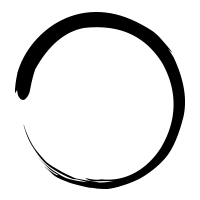
\includegraphics[width=\linewidth/4]{inzva-logo.png}
  \label{fig:inzva}
\end{figure}
\maketitle

\cleardoublepage
\tableofcontents
\markboth{Table of Contents}{}
\cleardoublepage
\newcommand{\sectionbreak}{\clearpage}

\section{Introduction}
\paragraph{}
In Graph-01 bundle, we were introduced to the basics of graph theory via a combination of definitions and concepts like DFS and BFS. We also learned about trees and tree-related data structures like heaps and BSTs. It is beneficial for the participants to recall the Graph-01 bundle before studying this bundle as some materials from the previous bundle are needed for this week's bundle.
\newline\newline
In this bundle, we will cover more in depth topics about graph theory. First we will cover some new definitions in graph theory, then we will move on the following topics:
\begin{itemize}
    \item Bipartite checking
    \item Topological sort
    \item Shortest path problem
    \item Minimum spanning trees
    
\end{itemize}
So let's move forward and discuss each topic in detail!

\section{Definitions}
\subsection{Bipartite Graphs}
\paragraph{}
A bipartite graph is a graph whose vertices can be divided into two disjoint and independent sets U and V such that every edge connects a vertex in U to one in V. Vertex sets U and V are usually called the parts of the graph. \cite{1}. The figure is shown in below. It is similar to graph coloring with two colors. Coloring graph with two colors is that every vertex have a corresponding color, and for any edge, it's vertices should be different color. In other words, if we can color neighbours two different colors, we can say that graph is bipartite.



\begin{figure}[h!]
\begin{center}
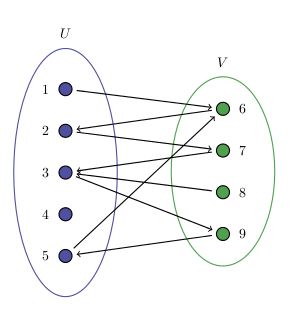
\includegraphics[width=\linewidth/2]{bipartite.png}
  \end{center}
\caption{ Example bipartite graph, all edges satisfy the coloring constraint }
  \label{fig}
\end{figure}


\paragraph{} We have some observations here.
\begin{itemize}
\item A graph 2- colorable if and only if it is bipartite. 
\item A graph does not contain odd-length cycle if and only if it is bipartite.
\item Every tree is a bipartite graph since trees do not contain any cycles. 
\end{itemize}

\newpage
\subsection{Directed Acyclic Graphs}
\paragraph{}
A directed acyclic graph(DAG) is a finite directed graph with no directed cycles. Equivalently, a DAG is a directed graph that has a topological ordering (we cover it in this bundle), a sequence of the vertices such that every edge is directed from earlier to later in the sequence \cite{2}. DAGs can be used to encode precedence relations or dependencies in a natural way \cite{4}. There are several applications using topological ordering directly such as finding  critical path or automatic differentiation on computational graphs (this is extremely useful for deep learning frameworks \cite{5}).  




\begin{figure}[h!]
\begin{center}
  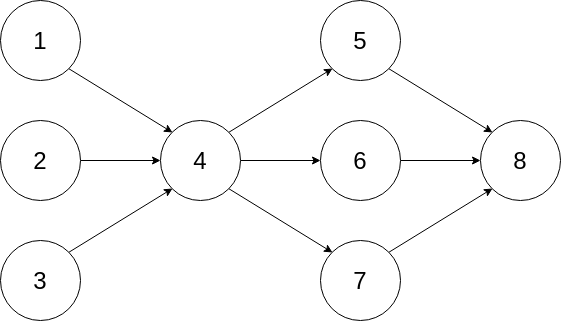
\includegraphics[scale = .7]{dag.png}
  \end{center}
\caption{Example Directed Acyclic Graphs}
  \label{fig}
\end{figure}



\begin{figure}[h!]
\begin{center}
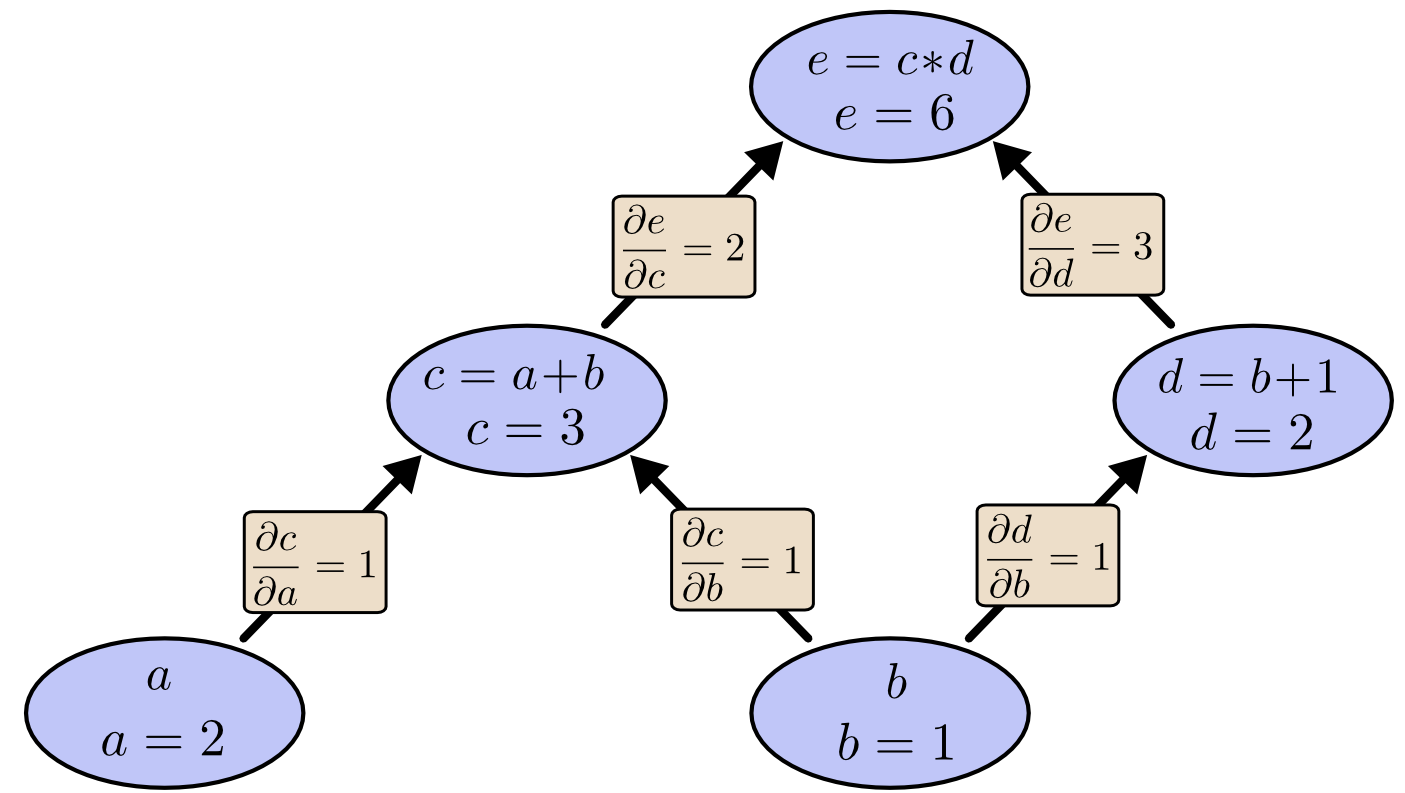
\includegraphics[scale = .25]{tree-def.png}    
 \end{center}
\caption{Example computational graph also a DAG, partial derivatives are written to edges respect to topological order}

  \label{fig}
\end{figure}



\section{Bipartite Checking}
\paragraph{}The question is in the title. Is the given graph bipartite? We can use BFS or DFS on graph. Lets first focus on BFS related algorithm. This procedure is very similar to BFS, we have an extra color array and we assign a color to each vertex when we are traversing the graph. Algorithm proof depends on fact that BFS explores the graph level by level. If the graph contains an odd cycle it means that there must be a edge between two vertices that are in same depth (layer, proof can be found on \cite{4}). Let's say the colors are red and black and we traverse the graph with BFS and assign red to odd layers and black to even layers. Then we check the edges to see if there exists an edge that its vertices are same color. If there is a such edge, the graph is not bipartite, else the graph is bipartite.
\begin{figure}[h!]
\begin{center}
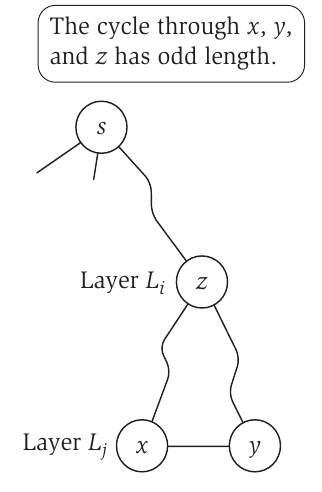
\includegraphics[scale =.8]{bipartite_check.png}    
  \end{center}
\caption{If two nodes x and
y in the same layer are joined
by an edge, then the cycle
through x, y, and their lowest
common ancestor z has odd
length, demonstrating that
the graph cannot be bipartite.
}
  \label{fig}
\end{figure}
\newpage
\begin{minted}{cpp}
typedef vector<int> adjList;
typedef vector<adjList> graph;
typedef pair<int,int> ii;
enum COLOR {RED, GREEN};
bool bipartite_check(graph &g){
    int root = 0; // Pick 0 indexed node as root.
    vector<bool> visited(g.size(),false);
    vector<int> Color(g.size(),0); 
    queue<ii> Q( { {root,0}} ); // insert root to queue, it is  first layer_0
    visited[root] = true;
    Color[root] = RED;
    while ( !Q.empty() )
    {
        /*top.first is node, top.second its depth i.e layer */
        auto top = Q.front();
        Q.pop();
        for (int u : g[top.first]){
            if ( !visited[u] ){
                visited[u] = true;
                //Mark even layers to red, odd layers to green
                Color[u] = (top.second+1) % 2 == 0 ?  RED : GREEN; 
                Q.push({u, top.second+1 });
            }
        }
    }
    for(int i=0; i < g.size(); ++i){
        for( auto v: g[i]){
            if ( Color[i] == Color[v] ) return false;
        }
    }
    return true;
}
int main(){
    graph g(3);
    g[0].push_back(1);
    g[1].push_back(2);
    g[2].push_back(3);
    cout << (bipartite_check(g) == true ? "YES" : "NO") << endl;
    return 0;
}
\end{minted}
\paragraph{}
The complexity of algorithm is is $O(V + E) + O(E) $, BFS and loop over edges. But we can say it  $O(V+E)$ since it is Big-O notation. \\ 
\section{Topological Sort}
\subsection{Definition}
\paragraph{}Topological sorting for Directed Acyclic Graph (DAG) is a linear ordering of vertices such that for every directed edge u->v, vertex u comes before v in the ordering. Topological Sorting for a graph is not possible if the graph is not a DAG \cite{6}.

\paragraph{}
 There are many important usages of topological sorting in computer science; applications of this type arise in instruction scheduling, ordering of formula cell evaluation when recomputing formula values in spreadsheets, logic synthesis, determining the order of compilation tasks to perform in makefiles, data serialization, and resolving symbol dependencies in linkers. It is also used to decide in which order to load tables with foreign keys in databases \cite{3}. 
 
 There are known algorithms (e.g Kahn's algorithm) to find topological order in linear time. Below, you can find one of the implementations:

\begin{figure}[h!]
\begin{center}
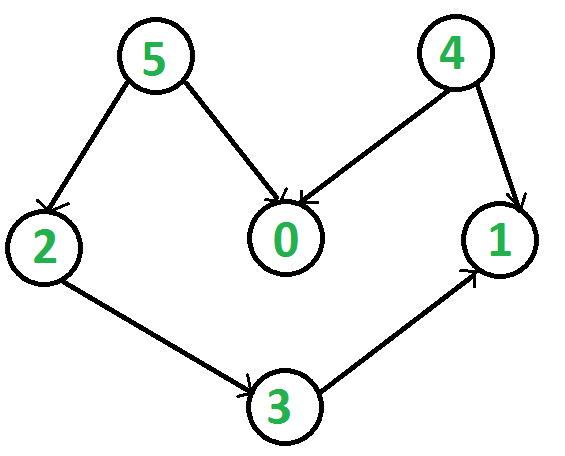
\includegraphics[width=\linewidth/2]{toporder.png}
  \end{center}
\caption{ For example, a topological sorting of this graph is “5 4 2 3 1 0”. There can be more than one topological sorting for a graph. For example, another topological sorting of the following graph is “4 5 2 3 1 0”. The first vertex in topological sorting is always a vertex with in-degree as 0 (a vertex with no incoming edges)\cite{6}.}
  \label{fig}
\end{figure}
\newpage
\subsection{Algorithm}
\begin{minted}{cpp}
typedef vector<int> adjList;
typedef vector<adjList> graph;
typedef pair<int,int> ii;
void kahn(graph &g){
    vector<int> result;
    queue<int> q;// 
    vector<int> degree(g.size(),0); // number of incoming egdes.
    for(auto &list: g){
        for(auto &node:list){
            degree[node]++;
        }
    }
    for(int i=0; i < g.size(); ++i){
        if (degree[i] == 0) q.push(i);
    }
    while( !q.empty()){
        int node = q.front();
        result.push_back(node);
        q.pop();
        for (auto &ng: g[node]){
            degree[ng]--;
            if ( degree[ng] == 0) q.push(ng);
        }
    }
    for(auto &i:result) cout << i << " ";
    cout << endl;
}
int main(){
    graph g(6);
    g[1].push_back(0);
    g[1].push_back(2);
    g[2].push_back(3);
    g[3].push_back(4);
    g[4].push_back(5);
    kahn(g);
    return 0;
}
\end{minted}
\paragraph{} As for time complexity: we traverse all edges in the beginning (calculating degrees) and in the while segment we remove edges (once for an edge) and traverse all nodes. Hence, the time complexity of this algorithm is $ O(V+E)$.
Note that this implementation assumes the graph is DAG. Try improving this code to support checking if the graph is DAG!
\section{Shortest Path Problem}
\subsection{Definition}
\paragraph{}
Let $G(V,E)$ be a graph, $v_i$ and $v_j$ be two nodes of $G$. We say a path between  $v_i$ and $v_j$ is the shortest path if sum of the edge weights (cost) in the path is minimum. In other words, the shortest path problem is the problem of finding a path between two vertices (or nodes) in a graph such that the sum of the weights of its constituent edges is minimized. \cite{7} 
\begin{figure}[h!]
\begin{center}
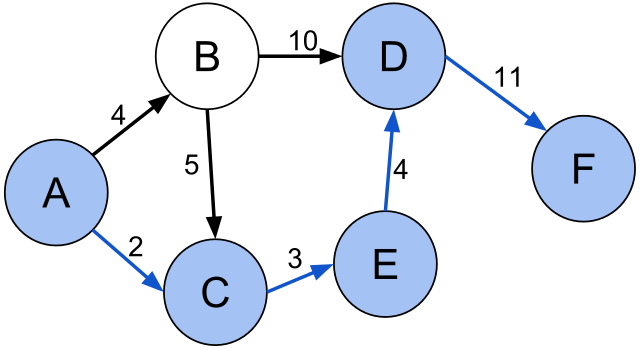
\includegraphics[width=\linewidth/2]{shortest.png}
  \end{center}
\caption{ Example shortest path in graph. Source is A and target is F. Image taken from \cite{7}.}
  \label{fig}
\end{figure}
\paragraph{}We will cover several shortest path algorithms in this bundle. One of them is Dijkstra's Shortest Path Algorithm but it has some drawbacks: Edge weights should be non-negative for the optimally of the algorithm. We will discover other algorithms in which these condition isn't necessary, like Floyd-Warshall and Bellman-Ford algorithms.
 \subsection{Dijkstra's Shortest Path Algorithm}
 \paragraph{}  Dijkstra's Shortest Path algorithm is straight forward. In brief we have a set $S$ that contains explored nodes and $d$ which contains the shortest path cost from source to another node. In other words, $d(u)$ represents the shortest path cost from source to node $u$. The procedure follows as that.
 First, add source node to set $S$ which represents the explored nodes and assigns the minimum cost of the source to zero. Then each iteration we add node to $S$ that has lowest cost $(d(u))$ from unexplored nodes. Let's say $S' = V-S$ which means unexplored nodes. For all nodes in $S'$ we calculate $d(x)$ for each node x is $S'$ then we pick minimum cost node and add it to $S$. So how we calculate $d(x)$?. For any $x$ node from $S'$, $d(x)$ calculated as that, let's say $e$ cost of any edge from $S$ to $x$ then $d(x) = min(d(u)+e)$. It is a greedy algorithm.

\newpage
\paragraph{}
Here is the explanation of the algorithm step by step.  

\begin{enumerate}
    \item Initialize an empty set, distance array, insert source to set.
    \item Initialize a min-heap, put source to heap with key is zero.
    \item While heap is not empty, take the top element from heap and add its neighbours to min-heap.
    \item Once we pick an element from the heap, it is guaranteed that the same node will never be added to heap with lower key value. 
\end{enumerate}

\paragraph{}
In implementatio,n we can use priority queue data structure in order to increase efficiency. If we put unexplored nodes to min - priority queue where the distance is key, we can take the lowest cost unexplored node in $O(log (n))$ time which is efficient. 
\begin{minted}{cpp}
typedef pair<int,int> edge;
typedef vector<edge> adjList;
typedef vector<adjList> graph;

void dijkstra(graph &g, int s){
    vector<int> dist(g.size(),INT_MAX/2);
    vector<bool> visited(g.size(),false); 
    dist[s] = 0;
    priority_queue<edge, vector<edge>, greater<edge>> q;
    q.push({0, s});
    while(!q.empty())
    {
        int v = q.top().second;
        int d = q.top().first;
        q.pop();
        if(visited[v]) continue;
        visited[v] = true;
        for(auto it: g[v])
        {
            int u = it.first;
            int w = it.second;
            if(dist[v] + w < dist[u])
            {
                dist[u] = dist[v] + w;
                q.push({dist[u], u});
            }
        }
    }
}
\end{minted}

\newpage
\subsection{Floyd-Warshall Algorithm}
\paragraph{}
The Floyd Warshall Algorithm is used for solving the all pairs shortest path problem. The problem is to find the shortest shortest distances between every pair of vertices in a given weighted directed graph \cite{8}. Instead of running Dijkstra's algorithm for every node as a source, Floyd-Warshall algorithm provides a simpler solution that uses the power of dynamic programming to achieve this task.
\paragraph{}


Lets state that in this algorithm, we have adjacency matrix representation of the graph. This algorithm works optimal even if there are negative edges but not negative cycles unlike the Dijkstra's shortest path. The algorithm looks for if any node can be an intermediate node for a path that decrease the cost. If the new cost is smaller, algorithm updates the cost in the adjacency matrix. For every k (as an intermediate node) in graph, we check all i,j pairs and we calculate $cost(i,k) +  cost(k,j)$.  Then we update $cost(i,j) $ with the new value if it is smaller than the current value.

\begin{minted}{cpp}
void floydWarshall (int graph[][V]) 
{ 
    /* dist[][] will be the output matrix that will finally have the shortest  
      distances between every pair of vertices */
    int dist[V][V], i, j, k; 
    /* Initialize the solution matrix same as input graph matrix. Or  
       we can say the initial values of shortest distances are based 
       on shortest paths considering no intermediate vertex. */
    for (i = 0; i < V; i++) 
        for (j = 0; j < V; j++) 
            dist[i][j] = graph[i][j]; 
    for (k = 0; k < V; k++) 
    { 
        for (i = 0; i < V; i++) 
        { 
            for (j = 0; j < V; j++) 
            { 
                if (dist[i][k] + dist[k][j] < dist[i][j]) 
                    dist[i][j] = dist[i][k] + dist[k][j]; 
            } 
        } 
    } 
} 
\end{minted}

\begin{figure}[h!]
\begin{center}
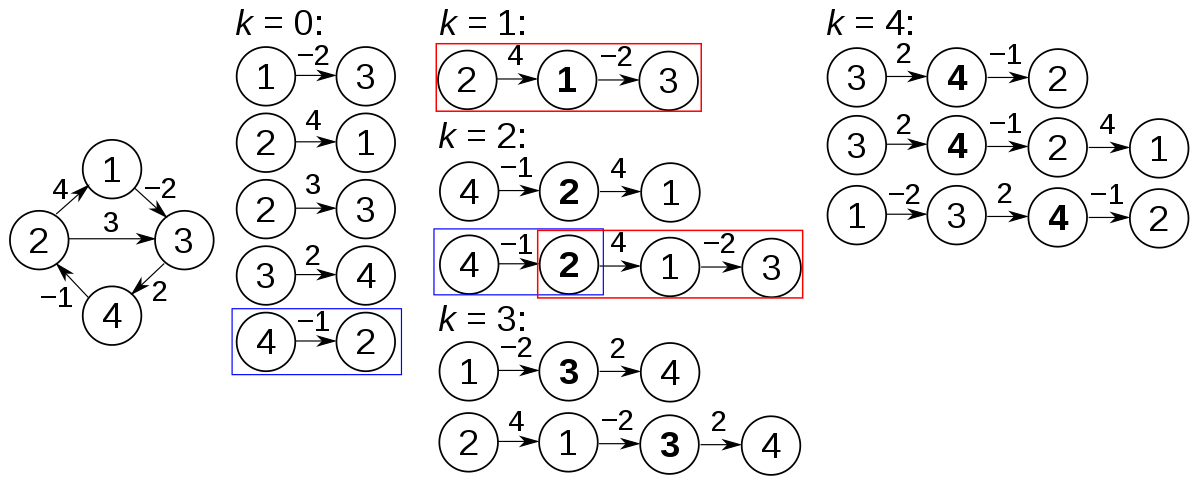
\includegraphics[scale=0.3]{floyd.png}
  \end{center}
\caption{ Example of Floyd-Warshall}
  \label{fig}
\end{figure}

\paragraph{} Time complexity of the algorithm can be seen here, there are three nested for loops over all nodes hence it is $O(V^3)$ and space complexity is $O(V^2)$ because we keep adjacency matrix in memory(after altering it with new values, it becomes a memoization table).

\subsection{Bellman Ford Algorithm}
\paragraph{}
The Bellman–Ford algorithm is an algorithm that computes shortest paths from a single source vertex to all of the other vertices in a weighted digraph. It is slower than Dijkstra's algorithm for the same problem, but more versatile, as it is capable of handling graphs in which some of the edge weights are negative numbers. Bellman-Ford algorithm also detects negative weighted cycles in the graph \cite{9}.

\paragraph{}
In this algorithm,  we maintain distance and the previous arrays to save costs and path. This algorithm is for single source shortest path problem and we initialize distance[source] to zero and all others to infinity. Then we check for all vertices in graph with all edges if using this edge makes the distance smaller than the current distance to this node. If it is smaller, we update distance and previous arrays. After constructing the previous and distance arrays, we loop over the edges and if we find a change on distance array, it means that graph contains a negative cycle. 

\begin{minted}{cpp}
typedef pair<int,pair<int,int>> edge;
typedef vector<edge> weigthed_graph;
void BellmanFord(weigthed_graph g, int V, int src) 
{ 
    int E = g.size(); 
    int dist[V]; 
    //this implemantation is just for negative cycle check
    // init distance array
    for (int i = 0; i < V; i++) 
        dist[i]   = INT_MAX; 

    dist[src] = 0; 
    for (int i = 1; i <= V-1; i++) 
    { 
        for (int j = 0; j < E; j++) 
        { 
            int u = g[j].second.first, v = g[j].second.second; 
            int weight = g[j].first; 
            if (dist[u] != INT_MAX && dist[u] + weight < dist[v]) 
                dist[v] = dist[u] + weight; 
        } 
    } 
    for (int i = 0; i < E; i++) 
    { 
        int u = g[i].second.first, v = g[i].second.second; 
        int weight = g[i].first;  
        if (dist[u] != INT_MAX && dist[u] + weight < dist[v]) 
            printf("Graph contains negative weight cycle"); 
    } 
}
\end{minted}


\paragraph{} There is a nested two for loops. One for vertices and one for edges so the time complexity of this algorithm is $O(EV)$. 
\begin{figure}[h!]
\begin{center}
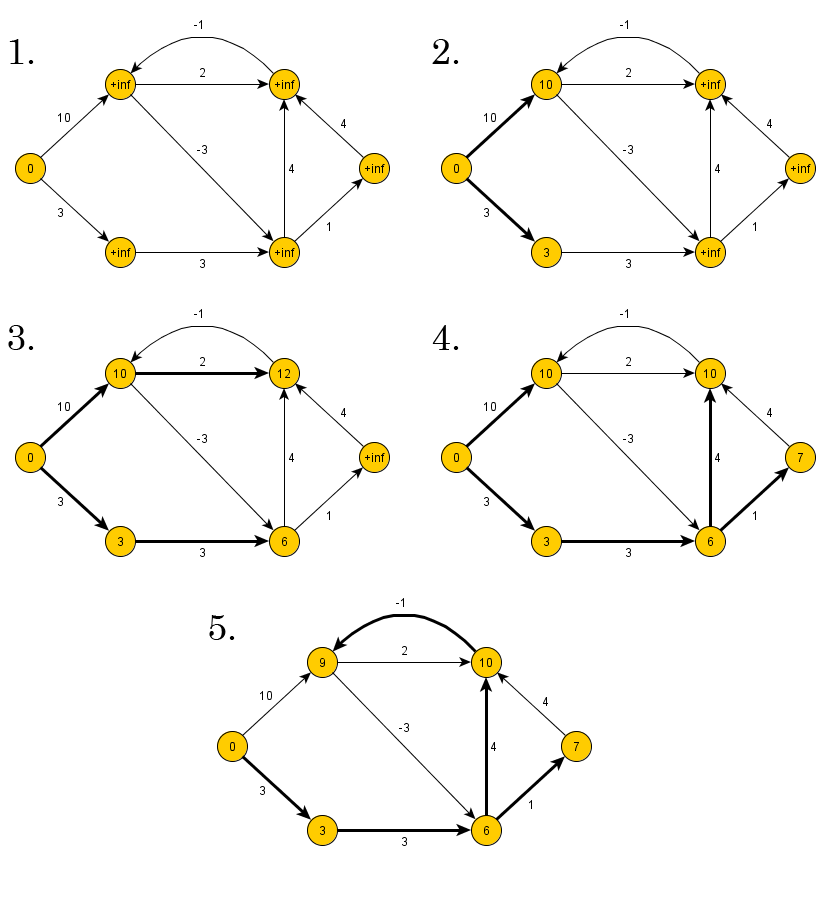
\includegraphics[width=\linewidth/3]{bellman.png}
  \end{center}
\caption{ Example of Bellman-Ford Algorithm }
  \label{fig}
\end{figure}
\newpage

\paragraph{} As a result, we inspected three shortest path algorithm. Here is a brief conclusion as a table.
\newline\newline
\begin{table}[]
\begin{tabular}{llll}
Algorithm                 & Time Complexity         & Space Complexity        & Notes                                    \\
 \hline
Dijkstra Shortest Path A. & $O(E logV)$             & $O(V^2)$                & 
\begin{tabular}{ll}Single Source \\ Fails on negative edges\end{tabular}  \\
 \hline
Floyd-Warshall A.         & $O(V^3)$ & $O(V^2)$ & 
\begin{tabular}{ll}All Pairs \\ Fails on negative cycle \end{tabular} \\
 \hline
Bellman-Ford A.           & $O(VE)$                   & $O(V+E)$                  & 
\begin{tabular}{ll} Single Source \\Can detect negative cycle \end{tabular} \\
 \hline
\end{tabular}
\end{table}

\section{Minimum Spanning Tree}
\subsection{Definition}
\paragraph{}
Given an undirected weighted connected graph  $G = (V,E)$ Spanning tree of G is a connected acyclic sub graph that covers all nodes and some edges. In a disconnected graph -where there is more than one connected component-  the spanning tree of that graph is defined as the forest of the spanning trees of each connected component of the graph. 
\paragraph{}
Minimum spanning tree (MST) is a spanning tree in which the sum of edge weights is minimum. The MST of a graph is not unique in general, there might be more than one spanning tree with the same minimum cost. For example, take a graph where all edges have the same weight, then any spanning tree would be a minimum spanning tree. In problems involving minimum spanning trees where you have to output the tree itself (and not just the minimum cost), it either puts more constraint so the answer is unique, or simply asks for any minimum spanning tree.

\begin{figure}[h!]
\begin{center}
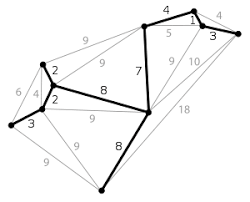
\includegraphics[width=\linewidth/3]{mst.png}
  \end{center}
\caption{ MST of the graph. It spans all nodes of the graph and it is connected. }
  \label{fig}
\end{figure}

To find the minimum spanning tree of a graph, we will introduce two algorithms. The first one called Prim's algorithm, which is similar to Dijkstra's algorithm. Another algorithm is  Kruskal agorithm, which makes use of the disjoint set data structure. Let's discover each one of them in detail!

\newpage
\subsection{Prim Algorithm}
\paragraph{}
Prim algorithm is very similar to Dijkstra's shortest path algorithm. In this algorithm we have a set $S$ which represents the explored nodes and again we can maintain a priority queue data structure the closest node in $V-S$. It is a greedy algorithm just like Dijkstra's shortest path algorithm. 

\begin{algorithm}[H]
\SetAlgoLined
  G = (V,E)   V  set of  all nodes \\
  T =  \{\}   result, edges of MST  \\
  S = { 1 };  explored nodes \\
 \While{S /= V}{
  let (u, v) be the lowest cost edge such that u in S and v in V - S; \\
    T = T U \{(u, v)\} \\
    S = S U \{v\}
 }
 \caption{Prim Algorithm in Pseudo code, what is the problem here? }
\end{algorithm}

\paragraph{} There is a problem with this implementation, it assumes that the graph is connected. If the graph is not connected this algorithm will be stuck on loop. There is a good visualization for Prim algorithm at \cite{10}. If we use priority queue complexity would be $O(ElogV)$ 

\begin{figure}[h!]
\begin{center}
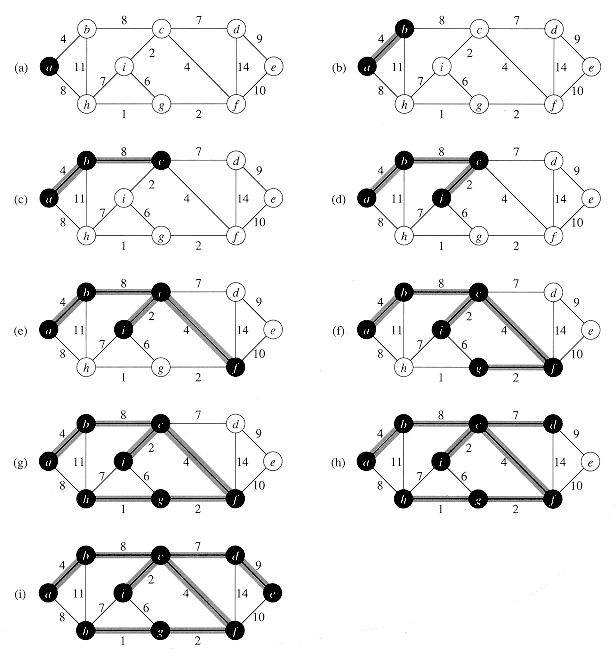
\includegraphics[width=\linewidth/2]{prim.png}
  \end{center}
\caption{ Example of how Prim Algorithm constructs the MST }
  \label{fig}
\end{figure}

\newpage
\subsection{Kruskal Algorithm}
In Prim algorithm we started with a specific node and then proceeded with choosing the closest neighbor node to our current graph. In Kruskal algorithm, we follow a different strategy;  we start building our MST by choosing one edge at a time, and link our (intially separated) nodes together until we connect all of the graph.
\newline\newline
To achieve this task, we will start with having all the nodes separated each in a group. In addition, we will have the list of edges from the original graph sorted based on their cost. At each step, we will:
\begin{enumerate}
    \item Pick the smallest available edge (that is not taken yet)
    \item Link the nodes it connects together, by merging their group into one unified group
    \item Add the cost of the edge to our answer
\end{enumerate}
% wait a minute, let me complete sth then I can explain ok


However, you may realize in some cases the link we add will connect two nodes from the same group (because they were grouped before by other taken edges), hence violating the spanning tree condition (Acyclic) and more importantly introducing unnecessary edges that adds more cost to the answer. So to solve this problem, we will only add the edges as long as they connect two currently (at the time of processing this edge) separated nodes that belong to different groups, hence completing the algorithm.
\newline\newline
The optimality of Kruskal algorithm comes from the fact that we are taking from a sorted list of edges. For more rigorous proof please refer to \cite{11}.
\newline\newline
So how can we effectively merge the group of nodes and check that which group each node belong? We can utilize disjoint set data structure which will help us to make union and find operations in an amortized constant $O(1)$ time. 
\begin{minted}{cpp}
typedef pair<int,pair<int,int>> edge;
// represent edge as triplet (w,u,v)
// w is weigth, u and v verticies.
// edge.first is weigth edge.second.first -> u, edge.second.second -> v
typedef vector<edge> weigthed_graph;

/*union - find data structure utilities */
const int maxN = 3005;
int parent[maxN];
int ssize[maxN];
void make_set(int v);
int find_set(int v);
void union_sets(int a, int b);
void init_union_find();

/*Code that finds edges in MST */
void kruskal(vector<edge> &edgeList ){
    vector<edge> mst;
    init_union_find();
    sort(edgeList.begin(),edgeList.end(), \
        [](const auto &a, const auto  &b) { return a.first< b.first;}); 
    //well this weird syntax is lambda function 
    // for sorting pairs to respect their first element.
    for( auto e: edgeList){
        if( find_set(e.second.first )!= find_set(e.second.second)){
            mst.push_back(e);
            union_sets(e.second.first, e.second.second);
        }
    }
}
\end{minted}

\paragraph{}
To calculate the time complexity, observe how we first sorted the edges, this takes $O(E log E)$. In addition we pass through the edges one by one, and each time we check which group the two nodes of the edge belongs to, and in some cases merge the two groups. So in the worst case we will assume that both operations (finding and merging) happens, but since the disjoint data structure guarantee $O(1)$ amortized time for both operations, we end up with $O(E)$ amortized time of processing the nodes.
\newline\newline
So in total we have $O(E log E)$ from sorting edges and $O(E)$ from processing them, those results in a total of $O(E log E)$ (if you don't understand why please refer to the first bundle where we discuss time complexity).


\begin{figure}[h!]
\begin{center}
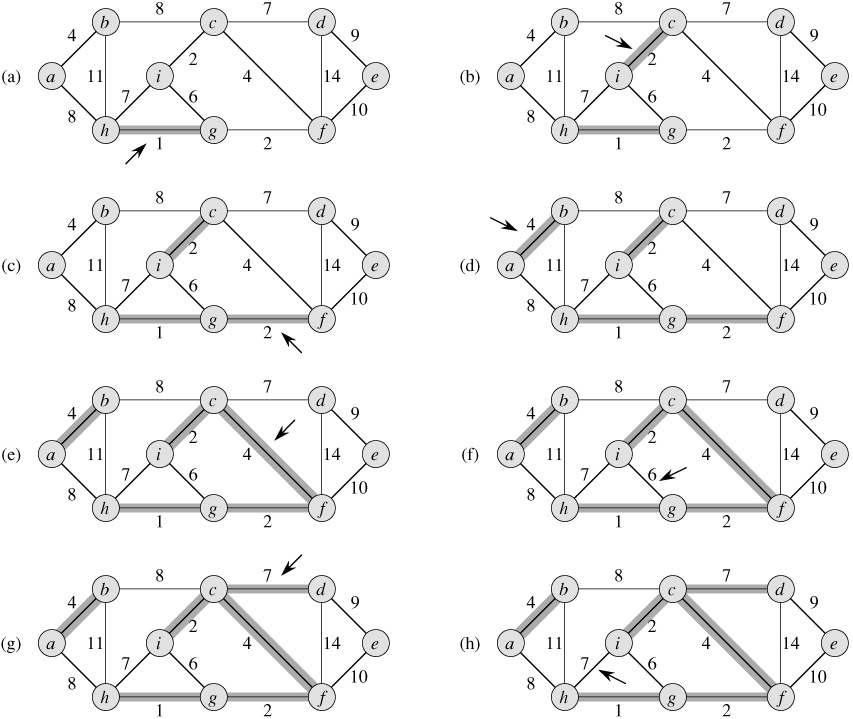
\includegraphics[width=\linewidth/2]{kruskal.jpg}
  \end{center}
\caption{ Example of how Kruskal Algorithm constructs the MST }
  \label{fig}
\end{figure}


% Ok here we go, there are several notes I wanted to say, I wanted to send an email, but since you're here I can simply write them here :D , ok?

%ok
% So first, I did some rephrasing to the paragraphs as you might noticed, btw did you review the changes or not yet? I discvored that you're here when your cursor was where I was writing, but I don't know how long have you been here :D, so 


% I checked the history I saw the most changest, I need to do floyd and belmman part, Havva is asking for it 
% Thx for kruskal part I did not have time at these days due to finals :/
 % yeah me too, I would like to help more, but I still have one final project to deliver before 7th which needs a lot of work, so I don't know if I work more on this , but in general, I would like to mention sth, try to simplify the language, the idea of explaining the problem in mathematical notation is good for someone who has a strong mathematical background, and I don't think that's the case for all people, I myself when I started programming I was always escaping those types of mathematical tutorials :D so I don't know whether we should do this or not, I tried to explain the kruskal algorithm in a different way to show you what I mean, I know it's not the best, but it's in simpler language, it's better to explain more here than to have strong mathematical notation since this course should be more of introductory, we might consider the fact that all those student are university students so this might help, but in general explaining the algorithm to someone who is new to it in mathematical notation would be some tedious in general cases, so I don't know, we might ask people at inzva for this but I would prefer to have more simple and longer explanations, The major issue is that time isn't in our favor. what do you think ???
 % I was not intent to make it math sugar I just used book as ref in dijktsra part and it happened :D, and it took  a lot of time for me also. Time is really strict, better verbal explanations would be better. I agree to you 
% But yeah still you did a great job specially in time of exams :D nobody likes to do sth else in these days, specially sth as time consuming as this, so let's put a plan, let's finish this reamaining section, then I can review them. 
% what's the deadline for this ???
% TODAY ??? OH: \ :| (
% Havva expecting it it before 6-7 pm for proofreading(a native person). TODAY :/. I just learnt it yesterday.. I will focus on reaminin parts now in more verbal and visual explanations.  ok, and I will try to help fix some of the past section if I have time. we better hurry up :\ :(
% Yes, did you review the Prim, it is too short how can make it longer, idk. , well I would rather explain disjktra more in verbal and detail as pseudo code, then prime can be a simple modification, as a matter of fact, we can convert dijkstra to prim code in one line :D so yeah it's so similar so we can depend on good explanation on dijsktra for that

% Okay I will add dijkstra pseudo code and more exp.. start with uncompleted parts first
% Okay
\newpage
\begin{thebibliography}{9}
\bibitem{1}
\href{https://en.wikipedia.org/wiki/Bipartite\_graph}{Bipartite Graph.  Wikipedia, the free online encyclopedia. Retrieved January 5, 2019}
\bibitem{2}
\href{https://en.wikipedia.org/wiki/Directed_acyclic_graph}{Directed Acyclic Graph.  Wikipedia, the free online encyclopedia. Retrieved January 5, 2019}
\bibitem{3}
\href{https://en.wikipedia.org/wiki/Topological_sorting}{Topological Sort. Wikipedia, the free online encyclopedia. Retrieved January 5, 2019} 
\bibitem{4}
Algorithm Design, Kleinberg, Tardos
\bibitem{5}
\href{ https://pytorch.org/docs/stable/autograd.html}{PyTorch AutoGrad website Depp Learning Framework}
\bibitem{6}
\href{https://www.geeksforgeeks.org/topological-sorting/}{Topological sort. Geeksforgeeks website. Retrieved January 5, 2019}
\bibitem{7}
\href{https://www.wikiwand.com/en/Shortest_path_problem}{Shortest Path. Wikipedia, the free online encyclopedia. Retrieved January 5, 2019}
\bibitem{8}
\href{https://www.geeksforgeeks.org/floyd-warshall-algorithm-dp-16/}{Floyd Warshall. Geeksforgeeks website. Retrieved January 5, 2019}
\bibitem{9}
\href{https://en.wikipedia.org/wiki/Bellman–Ford_algorithm}{Bellman Ford Wikipedia, the free online encyclopedia. Retrieved January 5, 2019}
\bibitem{10}
\href{https://www.wikiwand.com/en/Prim}{Prim Algorithm. Wikipedia, the free online encyclopedia. Retrieved January 5, 2019}
\bibitem{11}
\href{https://en.wikipedia.org/wiki/Kruskal%27s_algorithm}{Kruskal Algorithm. Wikipedia, the free online encyclopedia. Retrieved January 5, 2019}

\end{thebibliography}        
\end{document}
 